The domain model for the survey module is shown in Figure \ref{fig:survey_domainModel}.

\begin{figure}[htb]
\begin{center}
  %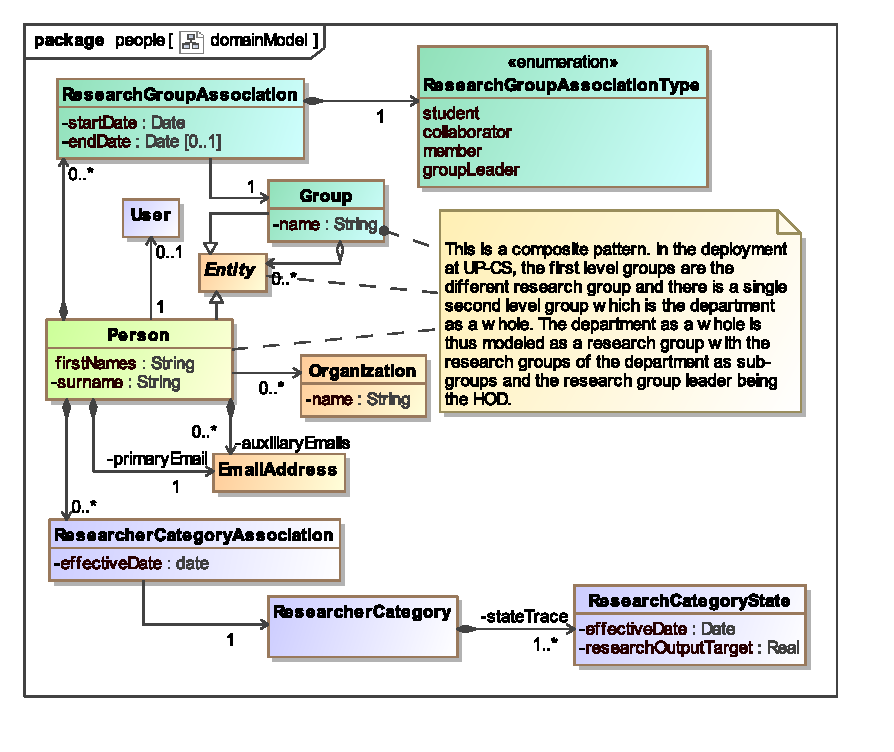
\includegraphics[width=0.8\textwidth,height=0.4\textheight,keepaspectratio=true]{domainModel}
\end{center}
\caption{ Domain model of the relations between entities forming the Survey module \label{fig:survey_domainModel}}
\end{figure}


A survey is a questionnaire. It typically consists of questions saved in a question bank. Different types of questions can be used, for example multiple choice, single field or paragraph. Read more about questions and question types in Section \ref{questions}. A questionnaire is a set of questions in a specified order.

A questionnaire is associated with zero or more rounds. If the current date is within the scope of the dates specified in an associated round, the questionnaire is active for the users in that active round. Read more about rounds in Section \ref{rounds}. 
